\documentclass[12pt,letterpaper]{article}
\usepackage{amsmath,amsthm,amsfonts,amssymb,amscd}
\usepackage{listings}
\usepackage{color}

\definecolor{dkgreen}{rgb}{0,0.6,0}
\definecolor{gray}{rgb}{0.5,0.5,0.5}
\definecolor{mauve}{rgb}{0.58,0,0.82}

\lstset{%frame=tb,
  language=Bash,
  aboveskip=3mm,
  belowskip=3mm,
  showstringspaces=false,
  columns=flexible,
  basicstyle={\small\ttfamily},
  numbers=none,
  numberstyle=\tiny\color{gray},
  keywordstyle=\color{blue},
  commentstyle=\color{dkgreen},
  stringstyle=\color{mauve},
  breaklines=true,
  breakatwhitespace=true
  tabsize=3
}

\usepackage{url}
\usepackage{caption}
\usepackage{subcaption}
\usepackage{graphicx}
\usepackage{wrapfig}
\usepackage{xcolor}
\usepackage[english]{babel}
\usepackage{mathtools}
\usepackage{fixltx2e}
\usepackage{hyperref}
\usepackage{enumerate}
\usepackage{fancyhdr}
\usepackage{mathrsfs}
\usepackage[margin=3cm]{geometry}
\setlength{\parindent}{0.0in}
\setlength{\parskip}{0.05in}

% Edit these as appropriate
\newcommand\course{CS595}
\newcommand\semester{FAll 2013}     
\newcommand\hwnum{7}
\newcommand\yourname{Amara Naas}
\newcommand\login{anaas}
\newcommand\DATE{11/8/2013}

\newenvironment{answer}[1]{
  \subsubsection*{Problem #1}
}

\pagestyle{fancyplain}
\headheight 40pt
\lhead{\yourname\ (\login)\\\course\ --- \semester}
\chead{\textbf{\Large Assignment \hwnum}}
\rhead{\DATE}
\headsep 40pt

\begin{document}

\begin{answer}{1}
In my approach to solve this problem I used the data from  \url {http://vlado.fmf.uni-lj.si/pub/networks/data/ucinet/zachary.dat} as specified in assignment 7. In order to use D3 as one of the assignment requirement I must convert the data from the url source to either JSON or CSV file since D3 can only handle these file type. In the file called {\it RScript.r}\footnote{File uploaded to github}:

\begin{itemize}
\item I imported the data from \url {http://vlado.fmf.uni-lj.si/pub/networks/data/ucinet/zachary.dat} and assigned it to "url" variable.
 \begin{verbatim}
url <- "http://vlado.fmf.uni-lj.si/pub/networks/data/UciNet/zachary.
dat"

\end{verbatim} 

\item By using the utilities in R I got the graph in pajek format and assigned it to a {\it graph} variable and than create a file called {\it table.txt}\footnotemark[1]. \par
\begin{verbatim}
graph <- graph.adjacency(l2, weighted=TRUE, mode="undirected")
write.graph(graph, "table.txt", format=c("pajek"))
\end{verbatim} 
\item I got the data needed from the table.txt file and add the names to the columns of the table so that I can save it as {\it JSON} file format.
\item I created a file in {\it JSON} format using the data before the graph splitting and called it {\it databefore.json}\footnotemark[1] file. 
\item I split the graph based on the maximum edge betweenness as defined by Girvan-Newman Algorithm. The function {\it edge.betweenness} in R calculates the edge betweenness as described in the following equation:
\end{itemize}
\begin{equation} \label{1}
E_B(e) = \sum_{{s\neq e}\neq t} g_{s_t}(e)/g_{s_t}
\end{equation}
where as:



\begin{flushleft}
g\textsubscript{st}(e) is total number of shortest paths from node s to node t.


g\textsubscript{st} is the number of those paths that pass through e.

\end{flushleft}
\begin{verbatim}
while loop ()
if (max==Edges[i+1])
		g <- delete.edges(g, E(g,get.edge(g,i)))
\end{verbatim}

\begin{itemize}
\item I save the data of the new created graph in the file called {\it table1.txt}\footnotemark[1] so I can convert this data and save it a {\it JSON} file format.
\begin{verbatim}
write.graph(graph, "table1.txt", format=c("pajek"))
\end{verbatim}

\item I created another file in {\it JSON} format using the data of the graph after the split and called it {\it dataAfter.json}\footnotemark[1] which contains the group member ship for each node.
\end{itemize}

I fed these files [{\it databefore.json} and {\it dataAfter.json}] to the D3 java script source which called {\it index.html}\footnotemark[1] in order to create a graph of the Karate club before and after the split. I built the java script source on top of the source from \url {http://bl.ocks.org/mbostock/4062045} and I got the {\it dragstart} function used in my source from \url {http://bl.ocks.org/mbostock/3750558}. Also I noticed that the code will not work if the source indexing starts from one, so I change the source indexing to starts from zero. The D3 source reads the data from the {\it JSON} files and creates nodes and links. The first graph can be created after opening the {\it index.html} file on the web browser and load the {\it databefore.json} as shown in Figure 1, and by clicking on the button on the browser the {\it dataAfter.json} file will be loaded and the graph will be split based on the \eqref{1} as shown in Figure 2.
\begin{verbatim}


\end{verbatim} 
\end{answer}

\begin{figure}
	\center
		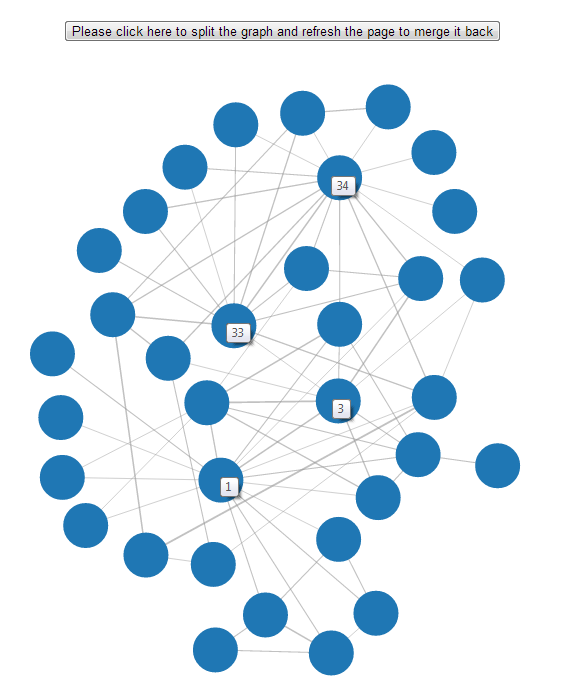
\includegraphics[width=\linewidth]{BeforeSplit.png} 
	\caption{Community Before Splitting}
\end{figure}
\begin{figure}
	\center
		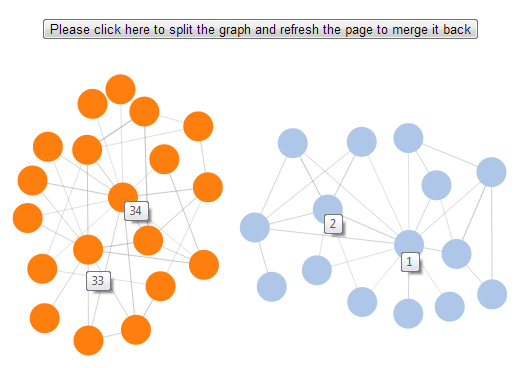
\includegraphics[width=\linewidth]{AfterSplit.png} 
	\caption{Community After Splitting}
\end{figure}

\end{document}
